\documentclass[12pt, a4paper]{article}
\usepackage{indentfirst}
\usepackage[backend=biber, citestyle=ieee]{biblatex}
\usepackage{ragged2e}
\usepackage{multicol}
\usepackage{graphicx}
\graphicspath{{./images/}}
\addbibresource{references.bib}
\title{Klasifikasi Kualitas Tidur Mahasiswa Berdasarkan Nilai Semester Satu Sampai Semester Lima Menggunakan Neural Network}
\author{Natan Hari Pamungkas}
\date{}

\begin{document}
\maketitle

\begin{abstract}
  %Todo = Write an abstract
\end{abstract}

Keywords: Data Mining, Neural Network, Sleep Quality

\section{Pendahuluan}
\begin{multicols}{2}
\justifying
Nilai mata kuliah adalah komponen penting bagi mahasiswa. Sebagian mahasiswa biasanya berusaha untuk menjaga nilai mata kuliah mereka agar minimal lulus sehingga tidak perlu mengulang. Nilai mata kuliah tiap semester ini juga yang akan mempengaruhi Indeks Prestasi Kumulatif (IPK) mahasiswa, dimana IPK akan digunakan untuk seleksi melamar pekerjaan. Meskipun bukan jaminan untuk mendapatkan pekerjaan, tapi IPK digunakan sebagai syarat administratif yang mutlak, sehingga jika IPK
kurang maka kemungkinan besar akan gagal untuk mendapatkan pekerjaan. \cite{Idris.2020}

Demi mengejar nilai yang baik, beberapa mahasiswa memiliki kebiasaan begadang. Tugas yang banyak membuat mahasiswa perlu mengorbankan waktu tidur untuk dapat menyelesaikannya. Semakin banyak tugas yang dapat diselesaikan dengan baik maka nilai mahasiswa juga akan semakin baik. \cite{Nielton.2019}

Kebiasan begadang demi meningkatkan nilai mata kuliah membuat mahasiswa mengalami kekurangan jam tidur. Hal ini disebabkan karena kebanyakan memiliki aktivitas di pagi sampai malam hari dan masih dilanjutkan untuk mengerjakan tugas sampai pagi hari lagi. Karena harus mengorbankan jam tidur untuk mengerjakan tugas, maka sebagian mahasiswa tidak dapat memenuhi kebutuhan jam tidur yang direkomendasikan, yaitu untuk usia 18-25 tahun adalah 7-9 jam. \cite{Hirshkowitz.2015}

Secara kesehatan, kekurangan jam tidur dapat menimbulkan masalah serius. Masalah-masalah tersebut dapat mempengaruhi baik fisik maupun mental seseorang. Masalah fisik yang dapat diderita oleh orang yang mengalami kekurangan jam tidur diantaranya adalah diabetes, kanker, dan penyakit jantung. Sedangkan masalah kesehatan mental yang dapat diderita diantaranya adalah \textit{anxiety}, depresi, dan insomnia. \cite{Berglund.2019}

Pada saat artikel ini ditulis, dunia terutama Indonesia sedang dalam perlawanan untuk melawan pandemi COVID-19. Penyakit yang disebabkan oleh virus SARS-CoV-2 ini pada tanggal 28 Mei 2020 telah menambah catatan jumlah pasien yang positif terinfeksi sebanyak 687 orang. Hal ini menandakan bahwa Indonesia masih dalam keadaan belum aman. \cite{Putri.2020} 

Hasil penelitian telah menemukan bahwa adanya korelasi antara obesitas dan COVID-19. Orang dengan obesitas memiliki resiko lebih tinggi untuk menderita pneumonia akut sebagai penyakit sekunder saat terinfeksi COVID-19. Hal ini membuktikan bahwa obesitas lebih rentan untuk menderita COVID-19 lebih parah dari orang dengan berat yang normal. \cite{Cai.2020}

Orang yang mengalami kekurangan jam tidur memiliki risiko yang tinggi untuk menderita obesitas. Hal ini disebabkan karena kekurangan tidur membuat tubuh seseorang mengalami hal-hal seperti resistensi terhadap hormon insulin sehingga tidak dapat mengatur kadar gula darah dengan baik, tidak dapat mengontrol nafsu makan karena disregulasi neuroendokrin, dan kurangnya aktifitas yang membakar energi. Hal ini tentu saja sangat berbahaya karena selain rentan terinfeksi COVID-19, orang
yang menderita obesitas juga memiliki risiko tinggi untuk menderita penyakit lain. \cite{Knutson.2007}

Selain masalah kesehatan, kekurangan jam tidur dapat mengakibatkan penurunan performa bekerja pada seseorang. Kehilangan jam tidur selama 17-19 jam memiliki efek yang sama saat seseorang mengkonsumsi alkohol hingga memiliki BAC (\textit{Blood Alcohol Content}) sebanyak kurang lebih 0,05 \%. Penurunan performa tentu saja membuat mahasiswa tidak dapat belajar di kelas dengan maksimal. \cite{Williamson.2000}

Usulan yang dapat diberikan oleh penulis adalah untuk menggunakan penelitian ini sebagai pengklasifikasi mahasiswa yang memiliki kekurangan tidur. Setelah diketahui mahasiswa-mahasiswa yang kemungkinan kekurangan jam tidur, selanjutnya dilakukan edukasi untuk memperbaiki jam tidur mereka. Hal ini karena berkaitan dengan masalah kesehatan dan tidak ada hubunganya antara prestasi belajar mahasiswa dan jam tidur. \cite{Sarfriyanda.2015}

\section{Studi Pustaka}
Paper ini ditulis berdasarkan paper terdahulu dengan judul "\textit{Sleep Quality Prediction From Wearable Data Using Deep Learning}". Pada paper tersebut, dilakukan penelitian untuk memprediksi kualitas tidur berdasarkan data yang diambil dari \textit{wearable devices}. Disini yang penulis ambil adalah memprediksi kualitas jam tidur berdasarkan data yang diisi selama perkuliahan menggunakan \textit{neural network}. \cite{Sathyanarayana.2016}

Objek penelitian yang digunakan oleh paper terdahulu adalah remaja-remaja di Qatar. Pengambilan data dilakukan oleh Weill Cornell Medical College-Qatar. Hal tersebut dilakukan untuk penelitian yang bertujuan untuk mencari korelasi antara pola tidur dengan berat badan pada remaja.

Metode penelitian pada paper terhadulu terdiri dari beberapa tahapan. Tahapan tersebut terdiri dari pengumpulan data, pemrosesan data, modeling data, dan evaluasi performa. Tahapan-tahapan tersebut dilakukan secara urut di dalam penelitian tersebut.

Pengumpulan data dilakuka dengan cara mengambil responden dari sekolah menengah atas kelas 7-11. Pengambilan data dilakukan selama satu minggu tanpa berhenti. Para responden menggunakan alat ActiGraph GT3X+ selama tujuh hari tanpa dilepas. Data dari alat tersebut dikumpulkan dan terdapat 322 data yang terdiri dari 102 data dari responden berjenis kelami laki-kali dan 220 data dari responden berjenis kelamin laki-laki. Total responden yang berpartisipasi pada penelitian ini ada 92
orang.

Pemrosesan data yang dilakukan ada beberapa tahap. Karena data yang didapatkan mengandung data dari \textit{triaxial accelerometer} dan data yang paling berpengaruh adalah data pada sumbu vertikal sehingga \textit{feature} adalah sumbu vertikal. Data yang masih multi dimensi ditransformasikan menjadi satu dimensi sehingga menjadi lebih sederhana dan mengurangi \textit{noise} di dalam data. Data yang berupa \textit{awake time} dan \textit{sleep time} digabungkan menjadi Unix
Epoch time untuk tiap-tiap menit. Data kosong yang diakibatkan dari pelepasan perangkat juga akan dihandle dengan cara dijadikan \textit{sleep time} maupun dihapus. 

Metode yang digunakan pada paper pendahulu adalah metode \textit{Deep Learning}. Metode tersebut juga dibandingkan dengan beberapa metode lainnya. Metode-metode lain yang digunakan sebagai pembanding adalah Logistic Regression, Multi-Layer Perceptrons (MLPs), Convolutional Neural Network (CNN), Recurrent Nerual Networks (RNN), Long short-term memory (LSTM) RNN, dan Time-Batched Long Short-Term Memory (TB-LSTM) RNN.

Logistic regression adalah sebuah metode statistika. Metode ini mampu mencari korelasi antara beberapa variabel independen dengan variabel dependen yang berlawanan. Model ini dapat memastikan bahwa kita akan selalu mendapatkan keluaran probabilistik antara 0 dan 1. \cite{Kleinbaum.2010}

Feed-forward neural network adalah sebuah arsitektur nerual network. Arsitektur ini membuat \textit{node} pada layer terhubung ke \textit{node} di layer atasnya, tetapi tidak terhubung ke \textit{node} di layer yang sama. Hal ini membuat informasi berjalan maju dan tidak melingkar. \cite{Schmidt.1992}

Multi-Layer Perceptrons adalah metode machine learning. Metode ini merupakan sebuah feed-forward neural network. Metode ini terdiri dari satu \textit{input} layer, beberapa \textit{hidden layers}, dan satu \textit{output} layer. \cite{Riedmiller.1994}

CNN adalah sebuah algoritma \textit{machine learning} yang terdiri dari input, output dan hidden layer, mirip seperti multi-layer perceptrons. Di dalam hidden layer CNN terdapat convolutional. Layer tersebut berguna untuk mengekstrak feature yang penting dari sebuah data. \cite{Valueva.2020}

RNN adalah algoritma \textit{machine learning} yang didesain mirip dengan sistem syaraf manusia. Jenis neural network ini termauk feed-forwarding neural network. Sesuai namanya, recurrent neural network ini memiliki \textit{activation} yang dapat terkoneksi secara recursive. \cite{Lukosevicius.2009}

LSTM adalah algoritma \textit{machine learning} yang berdasarkan pada RNN. Model ini memiliki kelebihan karena dapat mengatasi \textit{error backflow}. Hal ini dikarenakan algoritma gradient yang efisien membuat error flownya konstan. \cite{Hochreiter.1997}

\textit{Deep Learning} adalah algoritma pembelajaran mesin yang menggunakan metode pembelajaran representatif. Metode tersebut dilakukan dengan memproses data mentah menjadi representasi tingkat yang lebih tinggi. Hal ini membuat algoritma tersebut dapat menemukan pola yang akan digunakan untuk melakukan klasifikasi secara otomatis. \cite{LeCun.2015}

\section{Metodologi}
Dataset yang didapatkan merupakan hasil pengumpulan bersama mahasiswa-mahasiswa yang mengambil kelas Teknik Penambangan Data (TPD) tahun ajaran 2019/2020. Data yang dikumpulkan berupa nama, npm, nilai mata kuliah selama semester satu sampai semester lima, dan label-labelnya. Walaupun banyak label, namun hanya dipakai satu saja sesuai dengan judul penelitian.

\centering
\vspace{0.2cm}
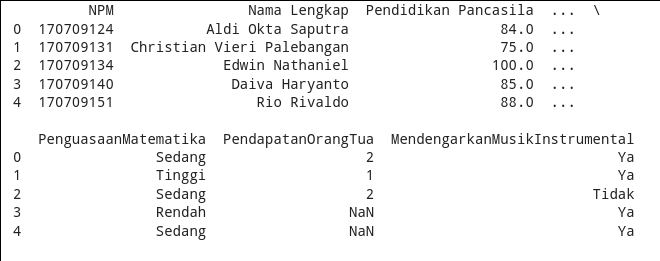
\includegraphics[scale=0.28]{see_data}
\vspace{0.2cm}

\justifying
Data yang sudah didapatkan kemudian dimuat ke dalam program. Data ini kemudian ditampilkan semua nama kolomnya dan informasinya. Kegunaanya adalah untuk mengeliminasi kolom yang tidak diperlukan seperti nama dan npm serta label-label yang tidak diperlukan. Hal ini berguna juga untuk melihat apakah ada data yang kosong atau tidak.

\centering
\vspace{0.2cm}
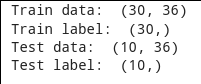
\includegraphics[scale=0.9]{split_test}
\vspace{0.2cm}

\justifying
Setelah dipastikan bahwa data besih dan dapat digunakan, maka selanjutnya bagi data ke dalam training dan testing secara acak. Pembagian ini dilakukan dengan porsi 75\% data training dan 25\% data testing. Hal ini dilakukan agar model dapat dilatih dan divalidasi menggunakan data yang berbeda. \cite{scikit-learn} 

\centering
\vspace{0.2cm}
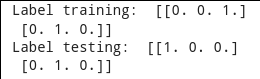
\includegraphics[scale=0.7]{encoded}
\vspace{0.2cm}

\justifying
Karena label masih berupa tipe data string seperti rendah, sedang, dan tinggi, maka perlu diubah ke bentuk numerik. Pengubahan menggunakan \textit{one-hot} encoding sehingga setiap label direpresentasikan menjadi \textit{list} yang merepresentasikan bilangan biner yaitu 0 jika tidak mengandung label tersebut dan 1 jika mengandung label tersebut. Urutan dari labelnya adalah mulai dari rendah, sedang, dan tinggi. Hal ini dikarenakan model tidak dapat memproses data yang bukan bertipe numerik.

\centering
\vspace{0.2cm}
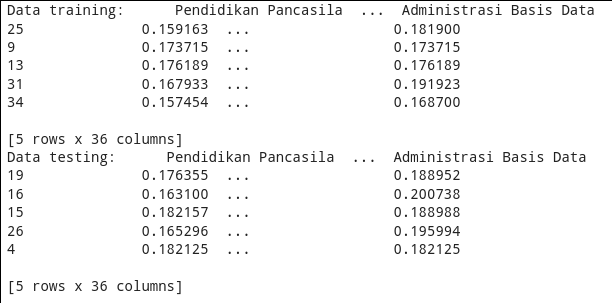
\includegraphics[scale=0.3]{normalize}
\vspace{0.2cm}

\justifying
Karena nilai yang terdapat data ada di pada jarak yang cukup besar, yaitu 0-100, maka perlu dilakukan normalisasi. Normaliasi ini mengubah data menjadi di dalam skala 0 sampai 1. Hal ini dilakukan agar model dapat memproses data dengan lebih baik dan lebih cepat. \cite{tensorflow2015-whitepaper}

\centering
\vspace{0.2cm}
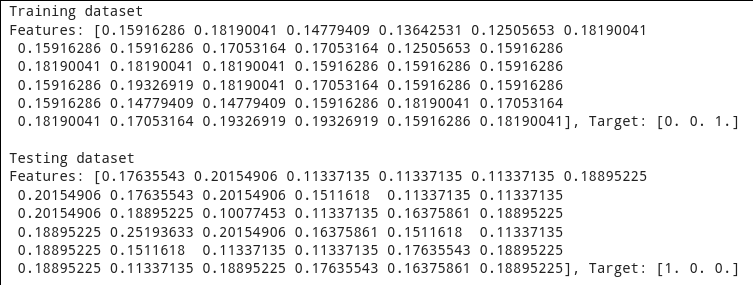
\includegraphics[scale=0.26]{dataset}
\vspace{0.2cm}

\justifying
Data yang sudah terproses kemudian diubah menjadi tensorflow dataset. Dataset ini terdiri dari data dan tiap-tiap labelnya. Hal ini bertujuan agar model dapat memproses data dengan mudah.

\centering
\vspace{0.2cm}
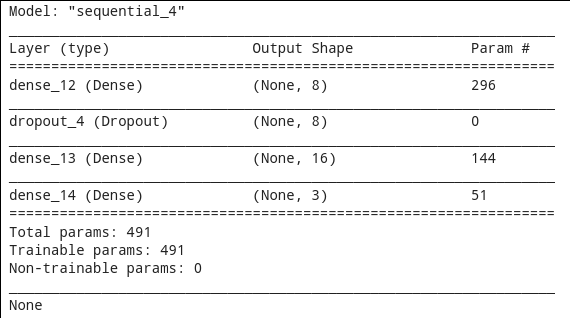
\includegraphics[scale=0.31]{model}
\vspace{0.2cm}

\justifying
Pada tahapan selanjutnya adalah pembuatan model. Disini menggunakan model \textit{sequential} dari tensorflow. Model ini menyusun tumpukan \textit{layer} secara sekuensial. Pada model ini digunakan tiga layer, yaitu satu \textit{input layer}, satu \textit{hidden layer}, dan yang terakhir \textit{output layer}. Pada \textit{input layer}, model menerima masukan data dengan dimensi (None, 36) dan mengeluarkan data dengan dimensi (None, 8). Selanjutnya adalah \textit{hidden layer} yang
menerima data dan mengeluarkan data dengan dimensi (None, 16). Dua layer diatas ini menggunakan aktivasi relu agar dapat belajar dengan cepat. Layer terakhir adalah \textit{output layer} yang menggunakan aktivasi softmax  dan mengeluarkan data dengan dimensi (None, 3). Fungsi softmax ini mengeluarkan prediksi dengan probabilitas, sehingga bentuk seluruh keluarnya probabilitasnya 100\%. Dalam pembuatan model ini menggunakan fungsi \textit{dropout} dengan nilai 0.5 yaitu mengeliminasi setengah
dari \textit{node} layer secara acak agar tidak terjadi \textit{overfitting}. 

\section{Result}

\centering
\vspace{0.2cm}
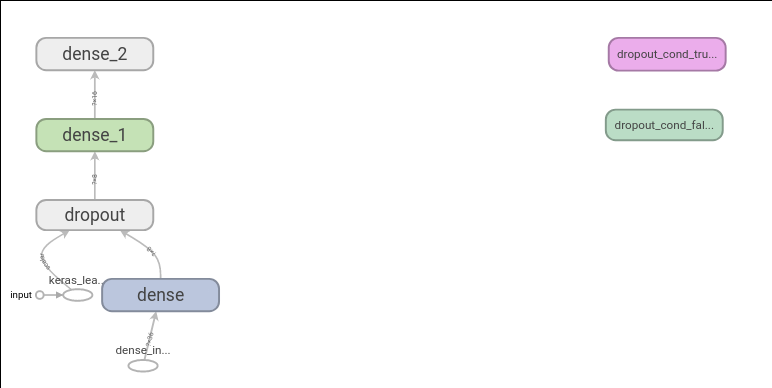
\includegraphics[scale=0.25]{model_graph}
\vspace{0.2cm}

\justifying
Gambar diatas merupakan hasil dari model. Terlihat bahwa ada tiga layer, namun tidak ditampilkan secara rinci. Di dalam grafik tersebut juga terdapat fungsi eperti \textit{dropout}.

\centering
\vspace{0.2cm}
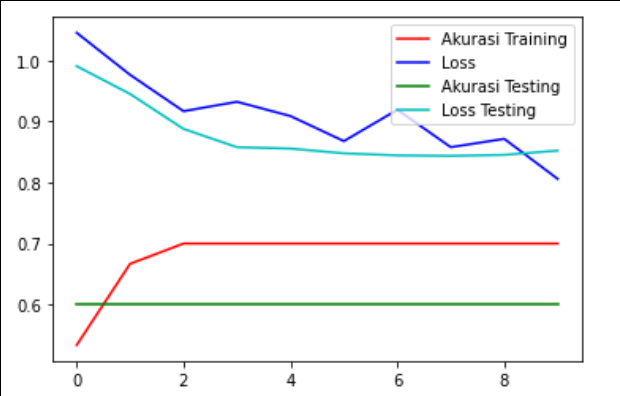
\includegraphics[scale=0.3]{acc}
\vspace{0.2cm}

\justifying
Hasil training pada model dapat dilihat pada grafik. Disitu terlihat bahwa \textit{loss} baik pada training maupun testing sudah mengalami penurunan. Pada bagian akurasi training mengalami kenaikan namun setelah mencapai 0.7 tidak lagi mengalami kenaikan. Sedangkan akurasi testing tidak mengalami perubahan, yaitu tetap 0.6. Hal ini menunjukan bahwa model mengalami \textit{overfitting}.

\centering
\vspace{0.2cm}
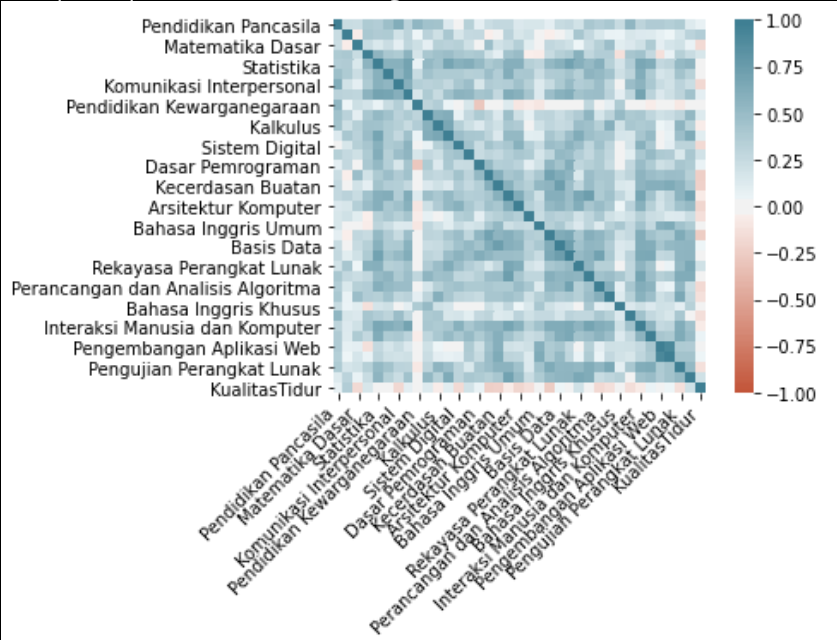
\includegraphics[scale=0.22]{heatmap}
\vspace{0.2cm}

\justifying
Karena model mengalami overfitting, maka harus melihat kembali data. Pada \textit{heatmap} tersebut terlihat korelasi antara \textit{features} dan label KualitasTidur. Terlihat bahwa tidak ada korelasi yang kuat antara nilai-nilai dengan kualitas tidur mahasiswa.

\section{Diskusi}
Penelitian ini menunjukan bahwa kualitas tidur tidak dipengaruhi oleh nilai mata kuliah mahasiswa dari semester satu samai semester lima. Hal ini ditunjukan dengan tidak adanya korelasi yang kuat antara nilai mata kuliah dengan kualitas tidur. Hal ini berbeda dengan penelitian yang pernah dilakukan pada paper terdahulu.

\end{multicols}

\newpage
\printbibliography[title = Daftar Pustaka]
\end{document}
